\documentclass[runningheads]{llncs}
%
\usepackage{graphicx}
% Used for displaying a sample figure. If possible, figure files should
% be included in EPS format.
\graphicspath{ {../plots/} }

\usepackage{calc}

% state diagrams
\usepackage{tikz}
\usetikzlibrary{automata, positioning, arrows}
\tikzset{
  initial text={},
  ->, % makes the edges directed
  node distance=3.0cm, % specifies the minimum distance between two nodes. Change if necessary.
  every state/.style={rectangle, thick, text width=5em, align=center}  % sets the properties for each ’state’ node
}

% tables
\usepackage{multirow}

\usepackage{hyperref}
% If you use the hyperref package, please uncomment the following line
% to display URLs in blue roman font according to Springer's eBook style:
\renewcommand\UrlFont{\color{blue}\rmfamily}

% references
\usepackage[numbers,sort]{natbib}

% quotation
\usepackage{dirtytalk}


\begin{document}

%
\title{Localised Reputation in the Prisoner's Dilemma}
%Spatial Prisoner’s Dilemma: \\
%Keep your enemies closer and be loud about it}
%
%\titlerunning{Abbreviated paper title}
% If the paper title is too long for the running head, you can set
% an abbreviated paper title here
%
\author{
Martin Toman \and
Neil Yorke-Smith\orcidID{0000-0002-1814-3515}\\\email{n.yorke-smith@tudelft.nl}
}
%
\authorrunning{M. Toman, N. Yorke-Smith}
% First names are abbreviated in the running head.
% If there are more than two authors, 'et al.' is used.
%
\institute{Delft University of Technology, The Netherlands}
%
\maketitle              % typeset the header of the contribution
%
%
%
\begin{abstract}
Under what conditions can cooperation emerge and be sustained?
Previous studies abstract cooperation and defection using the spatial Prisoner's Dilemma (PD) game.
%We build a computer simulation of a multi-agent spatial environment using Prisoner's Dilemma as the principal agent interaction.
We study a local reputation mechanism in which agents can remember defectors, abstain from interacting with them, and warn nearby agents.
%---local reputation of each agent is created.
Simulations find that local reputation is effective in sustaining cooperation and punishing defection.
Further, we find that the size of agent memory and amount of gossip are not significant factors, provided the locality range of gossip is greater than the agent movement speed.
%
%\keywords{First keyword  \and Second keyword \and Another keyword.}
\end{abstract}


%%%%%%%%%%%%%%%%%%%%%%%%%%%%%%%%%%%%%%%%%%%%%%%%%%%%%%%%%%%%%%%%%%%%%%%%%

\section{Motivation and Experimental Design}
%\section{Related Work \& Motivation}

Reputation systems strongly boost cooperation in spatial exchange games such as spatial PD \cite{simple-reputation, dong-reputation}.
Similarly, allowing game participants to pass information, either directly \cite{cooperation-communication} or indirectly \cite{public-private-monitoring}, increases the rate of cooperation.

We aim to explore the limits of local reputation---built up via gossip---in promoting and sustaining cooperation.
% in Spatial Prisoner’s Dilemma and under what parameters does it yield optimal results.
%
%
%
%\section{Methodology}
%We build a computer simulation \cite{smaldino} in Python using the Mesa\footnote{\url{https://github.com/projectmesa/mesa}} framework; the complete source is available online (\url{https://github.com/tinybeachthor/IPD}).
%
Agent's behaviour is defined by the finite state diagram shown in Figure~\ref{fig:agent_behaviour}.
We expand over prior work \cite{smaldino} %the model
by giving agents a (limited size) memory to keep track of defectors and to allow them to share this information by gossiping with other agents in a certain range.

\begin{figure}[tb]
  \centering
  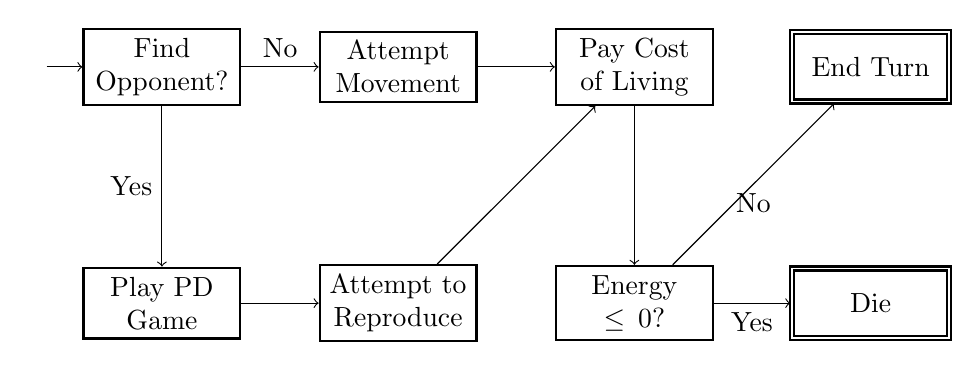
\begin{tikzpicture}

    \node[state, initial] (find_opponent) {Find Opponent?};

    \node[state, below of=find_opponent] (play) {Play PD Game};
    \node[state, right of=play] (reproduce) {Attempt to Reproduce};
    \node[state, right of=find_opponent] (move) {Attempt Movement};
    \node[state, right of=move] (cost) {Pay Cost of Living};
    \node[state, below of=cost] (energy) {Energy $\le 0$?};

    \node[state, accepting, right of=energy] (die) {Die};
    \node[state, accepting, above of=die] (end) {End Turn};

    \draw
      (find_opponent) edge[left] node{Yes} (play)
      (find_opponent) edge[above] node{No}  (move)
      (play) edge[] node{} (reproduce)
      (reproduce) edge[] node{} (cost)
      (move) edge[] node{} (cost)
      (cost) edge[] node{} (energy)
      (energy) edge[below] node{No}  (end)
      (energy) edge[below] node{Yes} (die)
      ;
  \end{tikzpicture}
  \caption{Agent behaviour diagram: showing the decision flow of an agent's single turn}
  \label{fig:agent_behaviour}
\end{figure}


%When running the simulation, we observe the saturation of cooperator and defector populations; we also record characteristic patterns \cite{spatial-patterns} formed by the populations as influenced by different parameters.
%These patterns are very similar to patterns occurring in nature, which are often created by reaction--diffusion processes.
%
%

\section{Results and Discussion}
We allow agents to remember the 5 most recent defectors and to ask nearby agents in a Moore neighbourhood of radius 1, 2, and 3 if they remember an agent defecting in a certain number of past encounters---varying between $0$ and $5$ (including both bounds).
We run the simulation for 1000 steps and plot the agent type saturations in Figure~\ref{fig:agent_sat/gossip_size_step1000}.

\begin{figure}[tb]
  \centering
  \makebox[\textwidth]{
    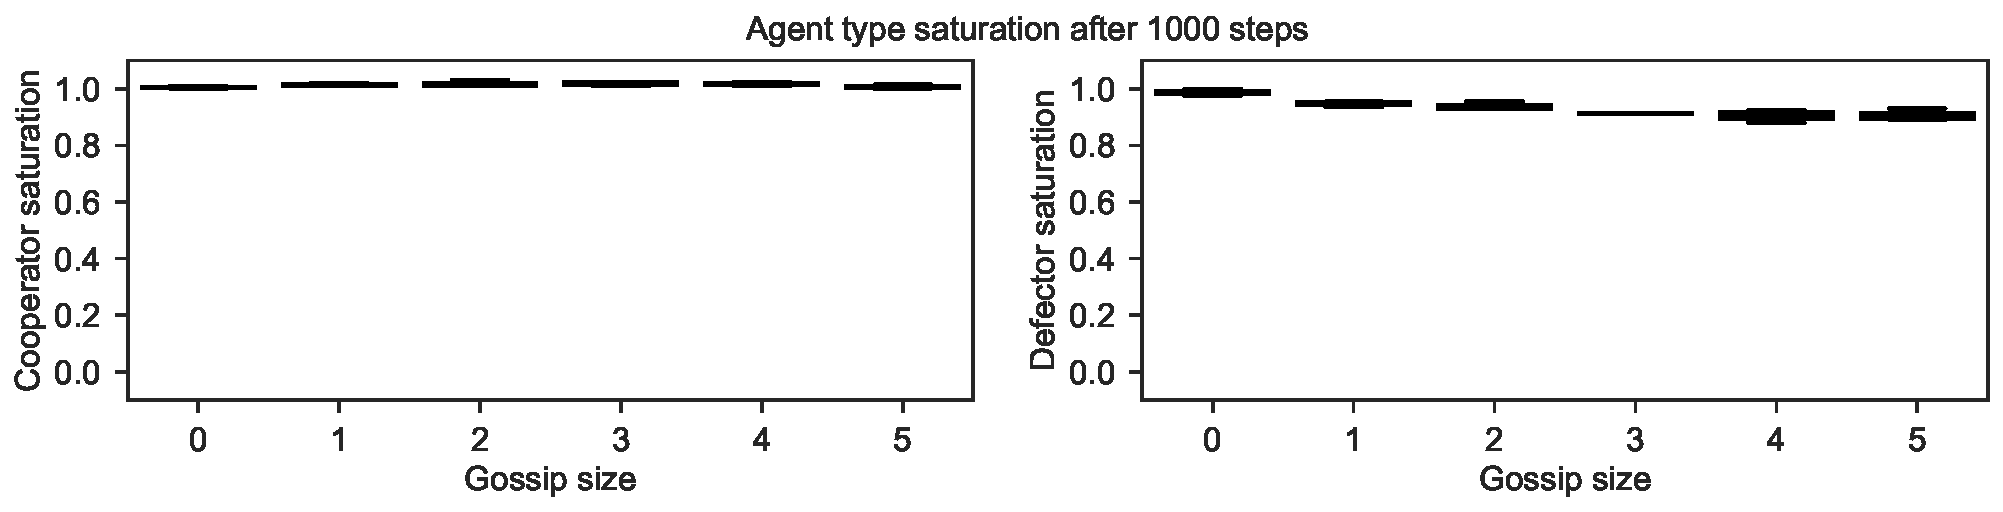
\includegraphics[width=\textwidth]{saturation&gossip_size-range1_1000steps_large.pdf}
  }
  \makebox[\textwidth]{
    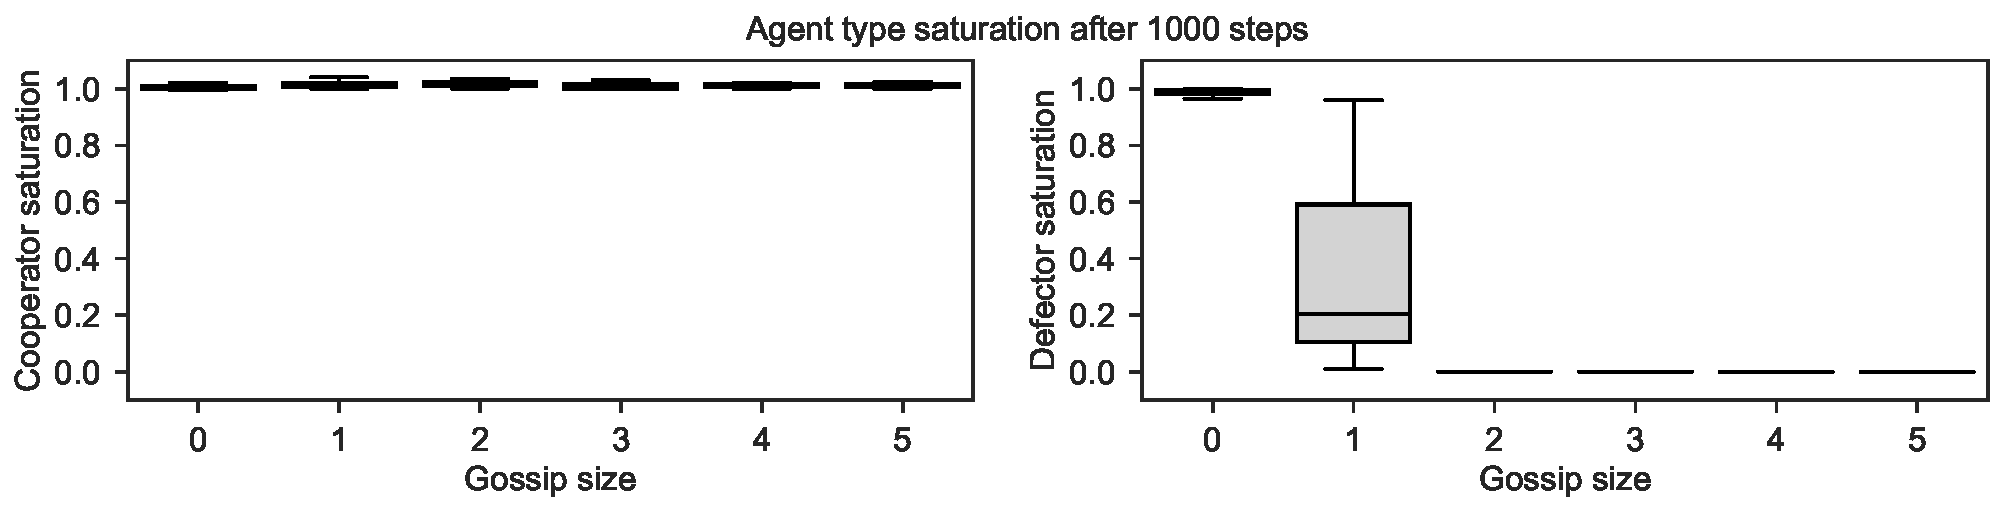
\includegraphics[width=\textwidth]{saturation&gossip_size-range2_1000steps_large.pdf}
  }
  \makebox[\textwidth]{
    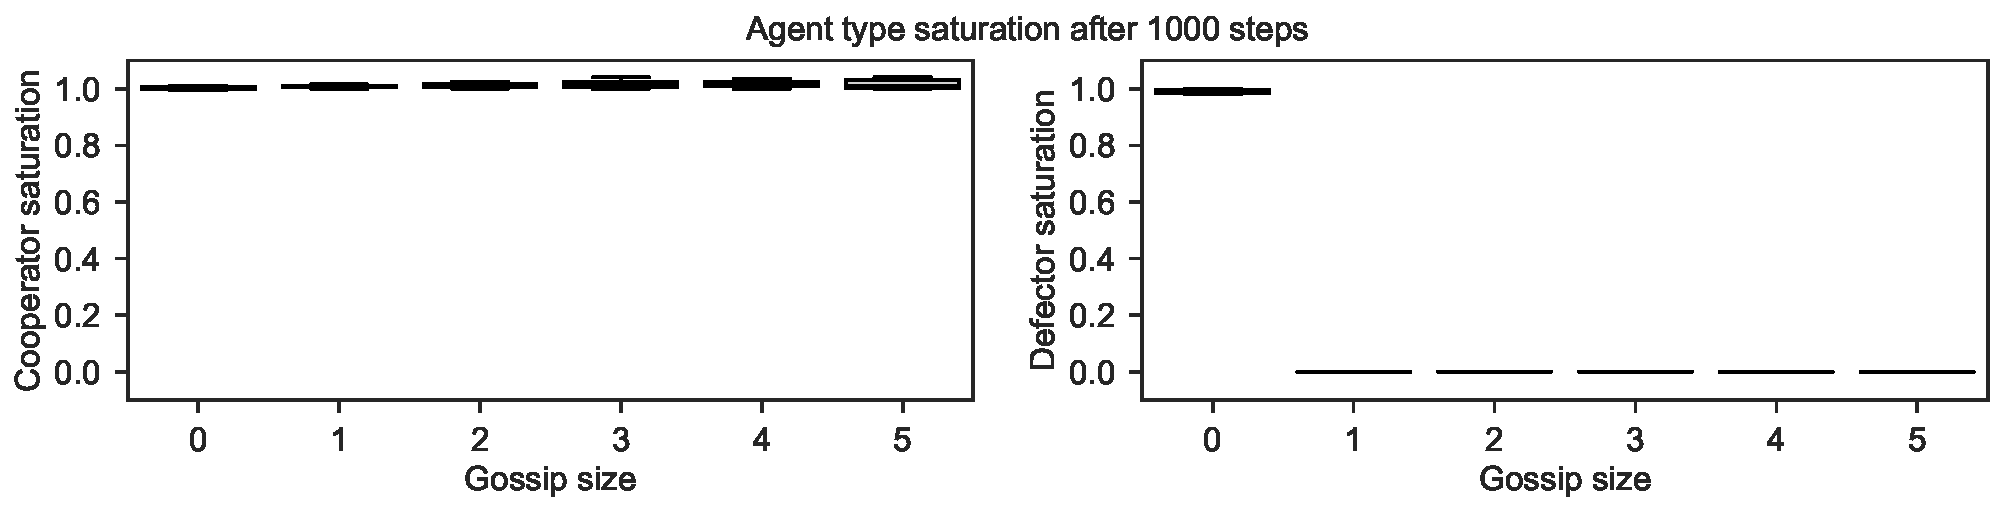
\includegraphics[width=\textwidth]{saturation&gossip_size-range3_1000steps_large.pdf}
  }
  \caption{Agent type saturation for various gossip sizes after 1000 steps, gossip radii 1, 2, and 3, respectively top to bottom; std.\@ dev.\@ of 30 simulation runs, outliers removed}
  \label{fig:agent_sat/gossip_size_step1000}
\end{figure}

The introduction of gossip is a strong deterrent of defection and quickly leads to cooperator--only populations.
The size of the memory and the size of the gossip are not significant factors, only speeding up the convergence slightly.
%The most important factor in predicting cooperator success is the range of the gossip.

%\begin{figure}[!hb]
%  \centering
%  \textbf{Baseline:} Memory size 0 - Gossip size 0 - Gossip range 0
%  \makebox[\textwidth]{
%    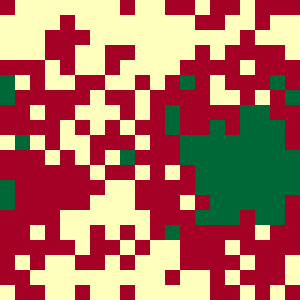
\includegraphics[width=\textwidth/4]{spatial-memory0+gossip0+range0.pdf}
%    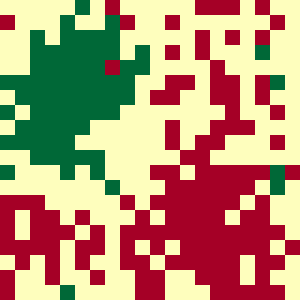
\includegraphics[width=\textwidth/4]{spatial-memory0+gossip0+range0-B.pdf}
%    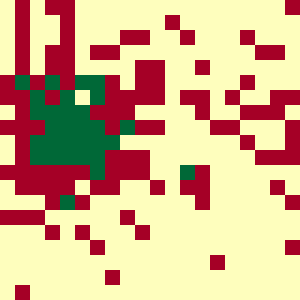
\includegraphics[width=\textwidth/4]{spatial-memory0+gossip0+range0-C.pdf}
%  }
%  \textbf{Final:} Memory size 1 - Gossip size 1 - Gossip range 3
%  \makebox[\textwidth]{
%    
\includegraphics[width=\textwidth/4]{spatial-memory1+gossip1+range3-A.pdf}
%    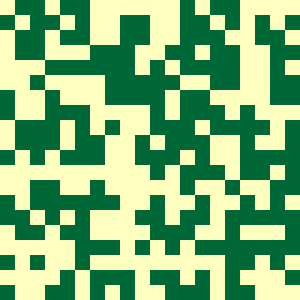
\includegraphics[width=\textwidth/4]{spatial-memory1+gossip1+range3-B.pdf}
%    
\includegraphics[width=\textwidth/4]{spatial-memory1+gossip1+range3-C.pdf}
%  }
%  \caption{Spatial patterns formed by agents after simulating for 500 steps, defectors shown in red, cooperators green, empty cells light-yellow}
%  \label{fig:spatial}
%\end{figure}

%We include images of the spatial patterns formed by the simulations in Figure~\ref{fig:spatial}.
%Since the model has an inspiration in biology this is an interesting visualization to include.


%\section{Conclusion}
Our simulation results find that the most important factor in predicting cooperator success is the range at which gossip can be exchanged; the amount of information included in the gossip has negligible effect.
If the gossip can move faster than agents, cooperators will flourish. Otherwise, defectors can reach full population saturation.
%The best way to ensure cooperation (and survival of a population) is to keep your enemies close and be loud about it. The louder the better.

% future work
Several directions can build on our results.
%Our simulation setup was limited in representing real world conditions.
Notably, we assumed all information is transferred with 100\% fidelity.  However,
not all strategies that perform well in noiseless environments can do so under the presence of noise~\cite{noise}.
The gossip mechanism could turn out to be disadvantageous if the agent behaviour was unpredictable enough, since it would deter more cooperator--cooperator interactions.



%%%%%%%%%%%%%%%%%%%%%%%%%%%%%%%%%%%%%%%%%%%%%%%%%%%%%%%%%%%%%%%%%%%%%%%%%

% ---- Bibliography ----
%
\renewcommand{\bibsection}{\section*{References}} % required for natbib to have "References" printed and as section*, not chapter*
\bibliographystyle{splncs04}
\bibliography{references}

\end{document}
